\chapter{Wstęp}
\section{Wprowadzenie}


Rozpowszechnione algorytmy sztucznej inteligencji wspomagające pracę inżynierów dźwięku można podzielić na dwie główne dziedziny \cite{analysis_generative} \label{traditional_algos}:

\begin{enumerate}
    \item algorytmy generujące symboliczny zapis nutowy (lub plik MIDI) (\ref{fig:lamus_notes}),
    \item algorytmy generujące gotowy plik audio (\ref{fig:riffusion_spectro}).
\end{enumerate}

Pierwsza grupa algorytmów znana jest już od lat 80, gdyż zagadnienie generowania zapisu symbolicznego jest mniej wymagające niż wytworzenie pełnego pliku audio. Powszechnie wykorzystywana jest w nich teoria muzyki, pozwalająca określić matematyczne relacje w rytmach, melodiach i progresjach akordów. Wiedza dotyczącą teorii muzyki pozwala na wyznaczenie możliwej przestrzeni stanów, w której generowana jest kompozycja, natomiast modele matematyczne takie jak łańcuchy markova służą za mechanizmy decyzyjne, które "nawigują" w przestrzeni stanów.

\begin{figure}[H]
    \centering
    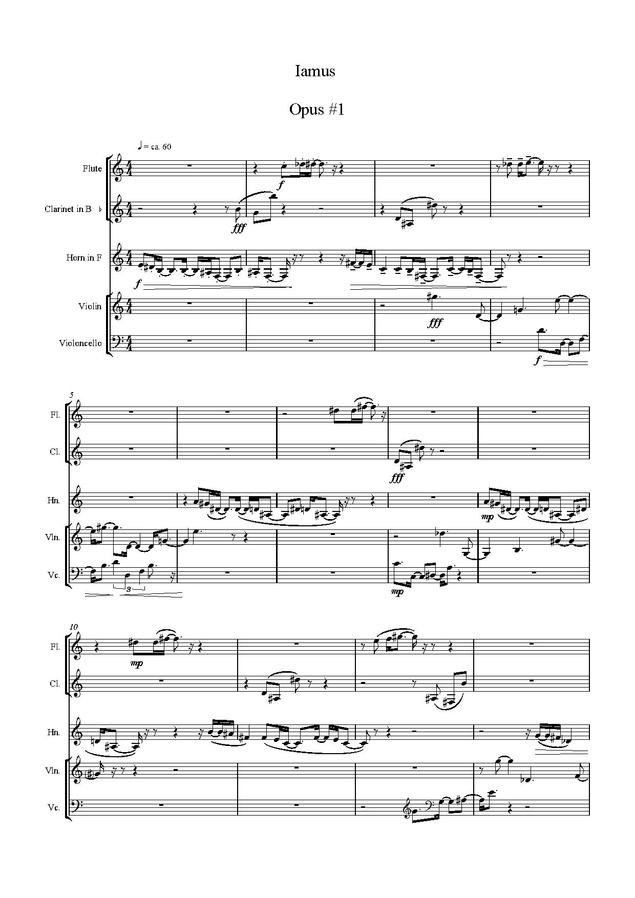
\includegraphics[width=0.4\linewidth]{rys01/lamus_notes.jpg}
    \caption{Zapis nutowy utworu \textit{Opus One}, wygenerowany przez komputer \textit{Lamus}.}
    \label{fig:lamus_notes}
\end{figure}

Druga grupa algorytmów, generująca gotowe nagrania, rozwija się korzystając z nowych możliwości, które zapewniają algorytmy z grupy stable diffusion \cite{stablediffusion}. Najnowsze projekty generujące pliki audio zgodne z opisem tekstowym (przykładowo   \texttt{"smutny jazz"} bądź \texttt{"muzyka taneczna w stylu Depeche Mode"}) szkolone są w taki sam sposób jak algorytmy stable diffusion. Zamiast na obrazach artystów, modele takie jak Stable Riffusion \cite{riffusion} szkolone są na spektrogramach, które następnie są w stanie wygenerować. Po wygenerowaniu spektrogramu przez model (\ref{fig:riffusion_spectro}), jest on konwertowany do pliku audio za pomocą odwrotnej transformaty Fouriera.

\begin{figure}[H]
    \centering
    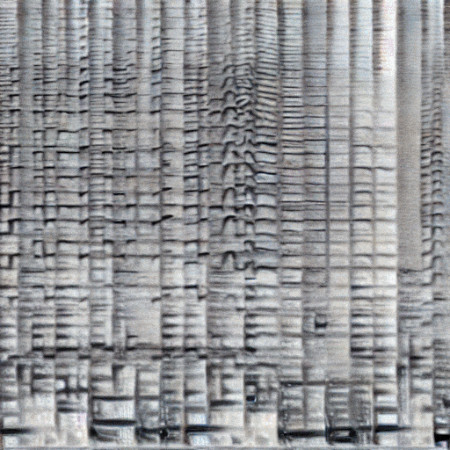
\includegraphics[width=0.4\linewidth]{rys01/riffusion_spectro.jpg}
    \caption{Przykładowy spektrogram wygenerowany przez algorytm \textit{Stable Riffusion} dla danych wejściowych \texttt{funk bassline with a jazzy saxophone solo}.}
    \label{fig:riffusion_spectro}
\end{figure}


% https://github.com/Kinyugo/msanii


Tematyka realizowanej pracy magisterskiej obraca się wokół zagadnień związanych z komputerową kompozycją i improwizacją, realizuje jednak zadanie, którego nie da się zaklasyfikować do żadnej z dwóch wyżej wymionionych dziedzin. Generowanie grafów przetwarzania
sygnałów dźwiękowych może być porównane z procesem projektowania instrumentu muzycznego.

Opisane wyżej (\ref{traditional_algos}) algorytmy pozwalają muzykowi lub inżynierowi
dźwięku na zainspirowanie się melodią lub wygenerowanym plikiem dźwiękowym.
Wynik pracy algorytmu implementowanego w ramach pracy magisterskiej jest \textbf{gotowym
instrumentem elektronicznym}, który może być wykorzystany w programie do komponowania
muzyki.


\section{Cel i zakres pracy}


Celem pracy jest zbadanie, czy algorytmy optymalizacyjne są w stanie samodziel-
nie wytworzyć graf przetwarzania sygnałów audio, który wykona syntezę próbki
dźwięku zadanej przez użytkownika.
Problem poruszany w pracy można zakwalifikować do grupy zagadnień związanych
z pojęciem \textit{computer-aided design} w dziedzienie inżynierii dźwięku. Docelowo
zaimplementowany algorytm będzie automatyzował pracę inżyniera dźwięku,
tworząc i konfigurując grafy przetwarzania sygnałów dźwiękowych, tak jak robi
się to w programach typu \textit{digital audio workstation} (Ableton, FL Studio).
Badania obejmują dwa zagadnienia:
\begin{enumerate} \label{research_types}
    \item metody generowania grafu przetwarzania sygnałów oraz późniejszej modyfikacji grafu,
    \item dobór funkcji błędu, na podstawie której algorytm optymalizujący będzie przeszukiwał
możliwą przestrzeń grafów przetwarzania sygnałów.
\end{enumerate}
Pierwsze zagadnienie sprowadza się do przetestowania szeregu algorytmów pozwalających na wygenerowanie
grafu przetwarzania sygnałów DSP oraz ich modyfikację (przykładem modyfikacji grafu
może być wprowadzanie w nim losowych zmian lub krzyżowanie dwóch grafów DSP w przypadku
wykorzystania algorytmu genetycznego).

Drugie zagadnienie obejmuje przetestowanie szeregu algorytmów, które można wykorzystać jako funkcję celu,
która będzie optymalizowana poprzez konfigurowanie grafu przetwarzania sygnałów dźwiękowych.



